\section*{Step 1}

\begin{custombox}[label={box:Q1}]{Step 1}
	Review the Jupyter Notebook \verb|E3.ipynb| and:
	\begin{enumerate}[label=(\alph*)]
		\item Create a summary of the code therein.
		\item Are there any learnings from this code that you wish to highlight?
	\end{enumerate}
\end{custombox}

\vspace{5mm}

This Python Notebook \verb|E3.ipynb| presents an analysis of various regression models applied to a dataset using polynomial features of different degrees. The models analyzed include Linear Regression, Support Vector Machine (SVM) Regression, Random Forest, Gradient Boosting, K-Nearest Neighbors (KNN), and Neural Networks. The performance of each model is evaluated based on metrics such as R-squared, Mean Squared Error (MSE), Durbin-Watson, and Jarque-Bera statistics. \\

We use the dataset given in \verb|E3-MLR3.xlsx|. The dataset contains $548$ samples of $(y, x_1)$ to train the model and $152$ samples of $(y, x_1)$ to test the model. 

\begin{figure}[H]
	\centering
	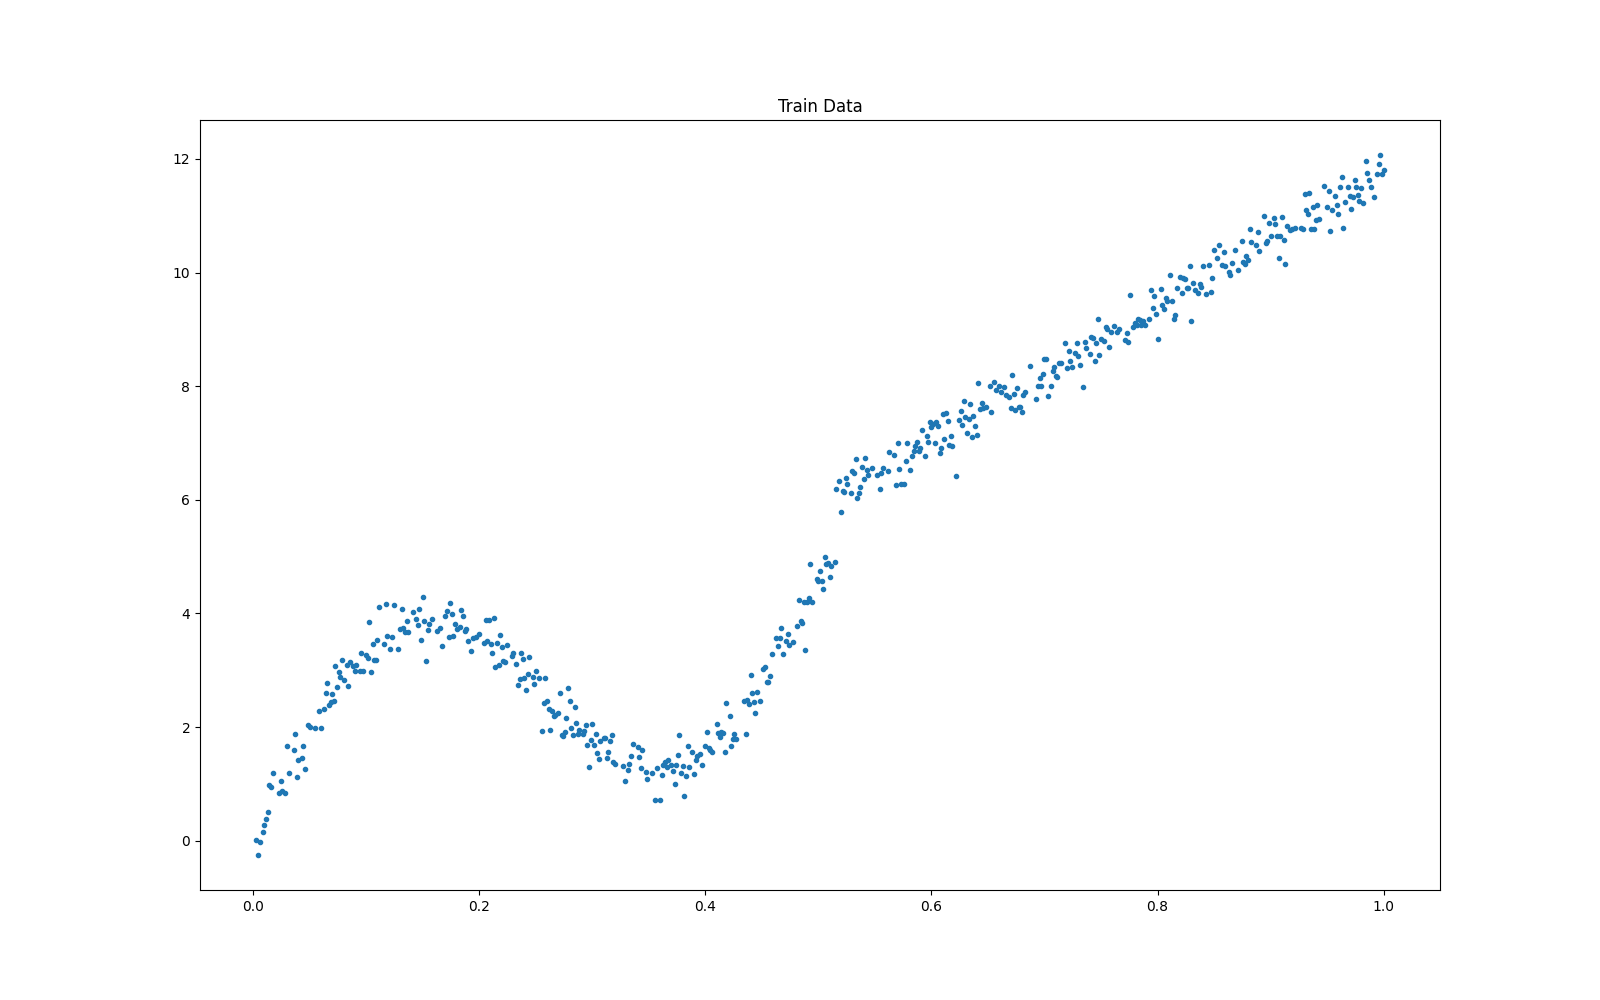
\includegraphics[width=0.7\linewidth]{./Images/E3-MLR3-Train.png}
	\caption{Training Data used in the analysis}
\end{figure}

\begin{figure}[H]
	\centering
	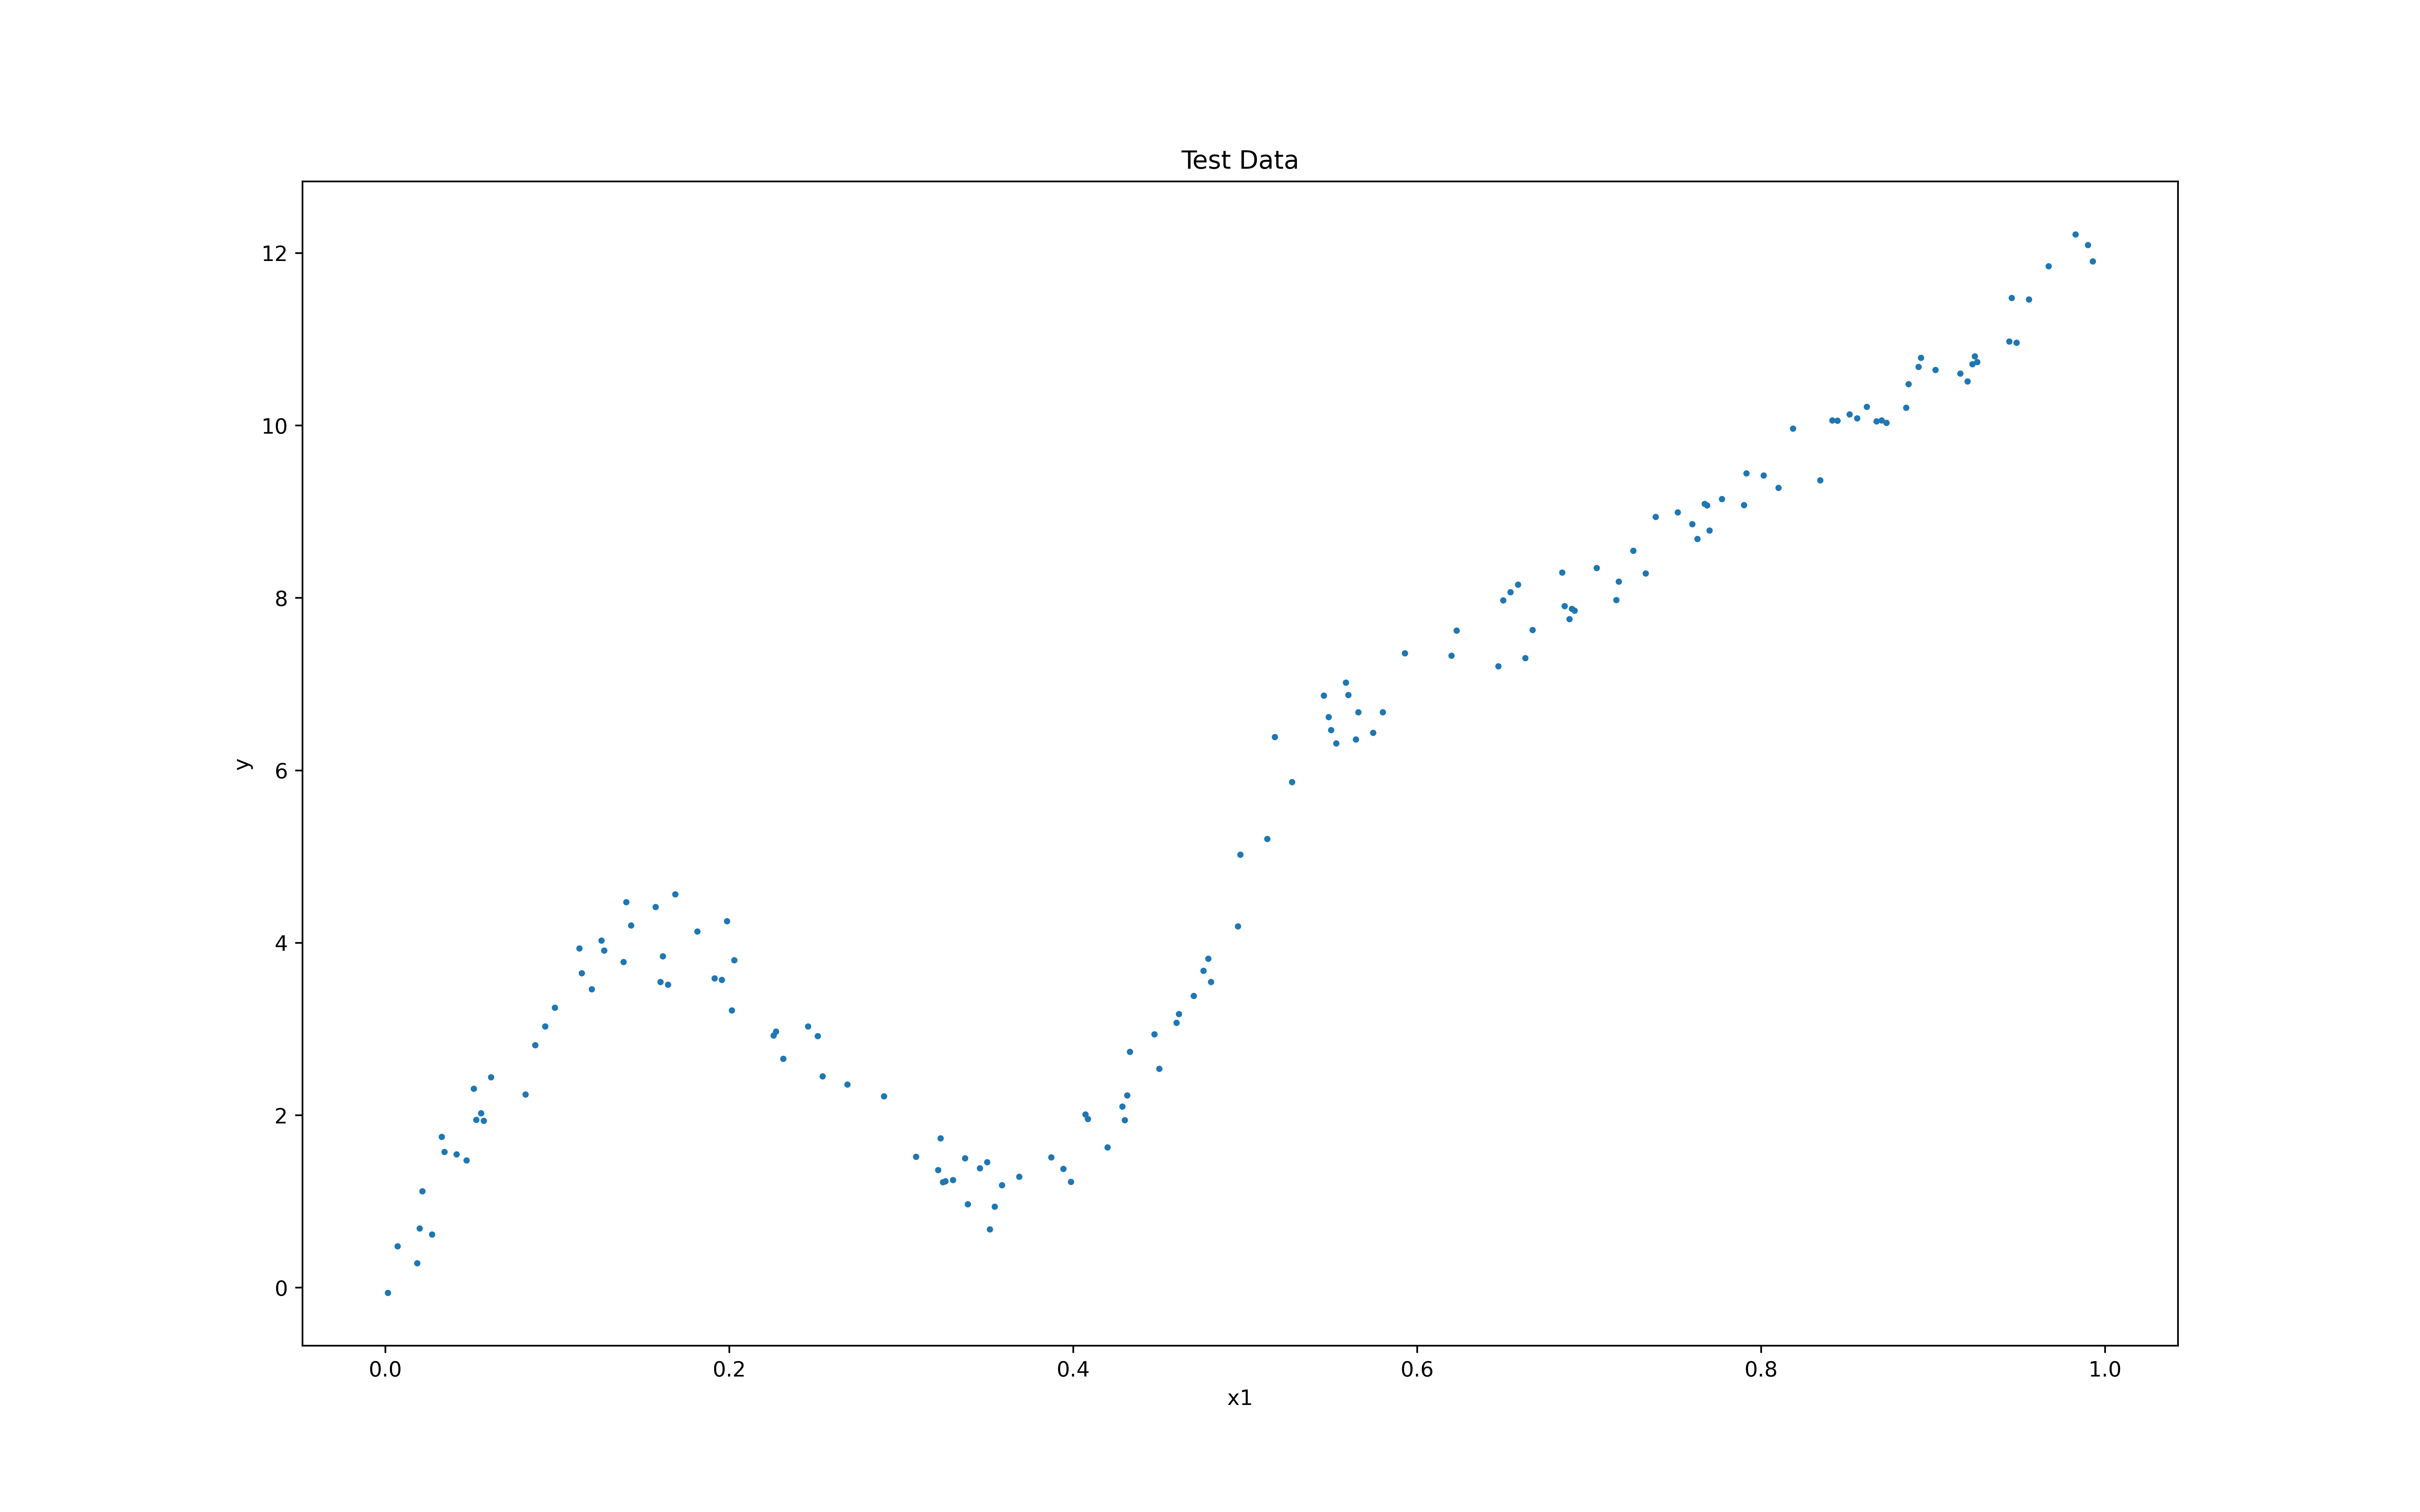
\includegraphics[width=0.7\linewidth]{./Images/E3-MLR3-Test.png}
	\caption{Testing Data used in the analysis}
\end{figure}

The following Python script in \verb|E3.ipynb| applies multiple regression algorithms to a dataset, evaluates their performance, and visualizes the results.

\subsection*{1. Importing Necessary Libraries}
\begin{lstlisting}[language=Python, caption={Importing Libraries}]
import pandas as pd
import numpy as np
from sklearn.preprocessing import PolynomialFeatures
from sklearn.linear_model import LinearRegression
from sklearn.svm import SVR
from sklearn.ensemble import RandomForestRegressor
from sklearn.ensemble import GradientBoostingRegressor
from sklearn.neural_network import MLPRegressor
from sklearn.neighbors import KNeighborsRegressor
from sklearn.metrics import mean_squared_error, r2_score
import statsmodels.api as sm
import matplotlib.pyplot as plt
\end{lstlisting}
\textbf{Description:} The code begins by importing essential libraries for data manipulation (\texttt{pandas}, \texttt{numpy}), machine learning models (\texttt{scikit-learn}), statistical analysis (\texttt{statsmodels}), and plotting (\texttt{matplotlib}).

\subsection*{2. Data Loading and Preprocessing}
\begin{lstlisting}[language=Python, caption={Loading and Preprocessing Data}]
file_path = 'E3-MLR3.xlsx'
train_data = pd.read_excel(file_path, sheet_name='train')
test_data = pd.read_excel(file_path, sheet_name='test')

X_train = train_data.drop(columns=['y'])
y_train = train_data['y']

X_test = test_data.drop(columns=['y'])
y_test = test_data['y']

poly = PolynomialFeatures(degree=6)
X_train_poly = poly.fit_transform(X_train)
X_test_poly = poly.transform(X_test)
\end{lstlisting}
\textbf{Description:} The script reads training and testing data from an Excel file and separates features (\texttt{X\_train}, \texttt{X\_test}) and the target variable (\texttt{y\_train}, \texttt{y\_test}). It then uses \texttt{PolynomialFeatures} to augment the features with polynomial terms of degree 6.

\subsection*{3. Saving the Augmented Dataset}
\begin{lstlisting}[language=Python, caption={Saving Augmented Data}]
feature_names = poly.get_feature_names_out(X_train.columns)
augmented_data = pd.DataFrame(X_test_poly, columns=feature_names)
augmented_data['y'] = test_data['y']
augmented_data.to_csv('augmented_data.csv', index=False)
\end{lstlisting}
\textbf{Description:} The code generates a CSV file containing the test data with the newly created polynomial features for review.

\subsection*{4. Defining and Running Regression Models}
\begin{lstlisting}[language=Python, caption={Defining and Running Regression Models}]
algorithms = {
    'Linear Regression': LinearRegression(),
    'SVM Regression': SVR(kernel='poly'),
    'RandomForest': RandomForestRegressor(),
    'XGBoost': GradientBoostingRegressor(),
    'knn': KNeighborsRegressor(),
    'Neural Network': MLPRegressor(hidden_layer_sizes=[10,10,10], max_iter=20000)
}

metric_table_train = pd.DataFrame()
metric_table_test = pd.DataFrame()

fig, axs = plt.subplots(len(algorithms), 4, figsize=(20, 20))
fig_row = -1

for algorithm_name, algorithm in algorithms.items():
    algorithm.fit(X_train_poly, y_train)
    y_train_pred = algorithm.predict(X_train_poly)
    y_test_pred = algorithm.predict(X_test_poly)

    r2_train = algorithm.score(X_train_poly, y_train)
    mse_train = mean_squared_error(y_train, y_train_pred)
    r2_test = algorithm.score(X_test_poly, y_test)
    mse_test = mean_squared_error(y_test, y_test_pred)

    residuals_train = y_train - y_train_pred
    residuals_test = y_test - y_test_pred

    durbin_watson_stat_train = sm.stats.durbin_watson(residuals_train)
    jb_stat_train, jb_p_value_train, _, _ = sm.stats.jarque_bera(residuals_train)
    
    durbin_watson_stat_test = sm.stats.durbin_watson(residuals_test)
    jb_stat_test, jb_p_value_test, _, _ = sm.stats.jarque_bera(residuals_test)

    metric_table_train.at[algorithm_name, 'R-squared'] = r2_train
    metric_table_train.at[algorithm_name, 'MSE'] = mse_train
    metric_table_train.at[algorithm_name, 'Durbin-Watson'] = durbin_watson_stat_train
    metric_table_train.at[algorithm_name, 'Jarque-Bera'] = jb_stat_train
    metric_table_train.at[algorithm_name, 'JB P-value'] = jb_p_value_train

    metric_table_test.at[algorithm_name, 'R-squared'] = r2_test
    metric_table_test.at[algorithm_name, 'MSE'] = mse_test
    metric_table_test.at[algorithm_name, 'Durbin-Watson'] = durbin_watson_stat_test
    metric_table_test.at[algorithm_name, 'Jarque-Bera'] = jb_stat_test
    metric_table_test.at[algorithm_name, 'JB P-value'] = jb_p_value_test

    fig_row = fig_row+1
    
    axs[fig_row, 0].scatter(train_data['x1'], y_train)
    axs[fig_row, 0].scatter(train_data['x1'], y_train_pred)
    axs[fig_row, 0].set_title(algorithm_name + " - Train")
    
    axs[fig_row, 1].scatter(train_data['x1'], residuals_train)
    axs[fig_row, 1].set_title(algorithm_name + " Residuals - Train")
    
    axs[fig_row, 2].scatter(test_data['x1'], y_test)
    axs[fig_row, 2].scatter(test_data['x1'], y_test_pred)
    axs[fig_row, 2].set_title(algorithm_name + " - Test")
    
    axs[fig_row, 3].scatter(test_data['x1'], residuals_test)
    axs[fig_row, 3].set_title(algorithm_name + " Residuals - Test")
\end{lstlisting}
\textbf{Description:} A dictionary of regression algorithms is created. Each algorithm is trained on the polynomial features, and its performance is evaluated using metrics such as R-squared, Mean Squared Error (MSE), Durbin-Watson, and Jarque-Bera test. These metrics are stored in tables. The residuals and predicted values are also plotted.

\subsection*{5. Visualizing the Results}
\begin{lstlisting}[language=Python, caption={Visualizing the Results}]
plt.tight_layout()
plt.show()
\end{lstlisting}
\textbf{Description:} The code concludes with displaying the generated plots for each regression model.

\subsection*{6. Plotting Error Metrics}
\begin{lstlisting}[language=Python, caption={Plotting Error Metrics}]
print("Metrics - Train Data:\n")
print(metric_table_train.to_string())
print("-------------------------------------------------")

print("Metrics - Test Data:\n")
print(metric_table_test.to_string())
print("-------------------------------------------------")
\end{lstlisting}

\textbf{Description:} The code prints the error metrics for each regression model on both training and testing datasets.

\subsection*{Learnings from this Code}

\begin{enumerate}[label=(\alph*)]
	\item The code demonstrates the application of various regression algorithms to a dataset with polynomial features.
	\item It highlights the importance of evaluating regression models using multiple metrics to understand their performance.
	\item The code showcases the use of residual analysis to assess the model's assumptions and identify potential issues.
	\item It provides a structured approach to comparing different regression models and their outcomes.
	\item The code emphasizes the significance of visualizing the model's predictions and residuals for better interpretation.
	\item The code also shows how to save augmented datasets for further analysis or review.
\end{enumerate}

\clearpage